% Dmitry Mikushin, UNIL, dmitry@kernelgen.org

\documentclass[aspectratio=169,twoside]{beamer}

\usetheme{unil}
\usepackage{comment}
\usepackage{enumerate}
\usepackage{xcolor}
\usepackage{setspace}
\usepackage{mathrsfs}
\usepackage{multibbl}
\usepackage{relsize}
\usetikzlibrary{calc,shapes.callouts,shapes.arrows}

\title[HPC Multi-iterator Engine]{HPC Multi-iterator Engine\\ Design \& Implementation}
\author[Dmitry Mikushin et al.]{Dmitry Mikushin\quad Simon Scheidegger\\ Philipp Eisenhauer\quad Moritz Mendel}
\institute[UNIL]{}
\date{May 4, 2021}



\begin{document}



{
\setbeamertemplate{footline}{} 
\begin{frame}
  \titlepage
\end{frame}
}
\addtocounter{framenumber}{-1}



\setbeamercovered{transparent=5}



\begin{frame}[fragile]{Multi-Iterator: the purpose}

\begin{center}
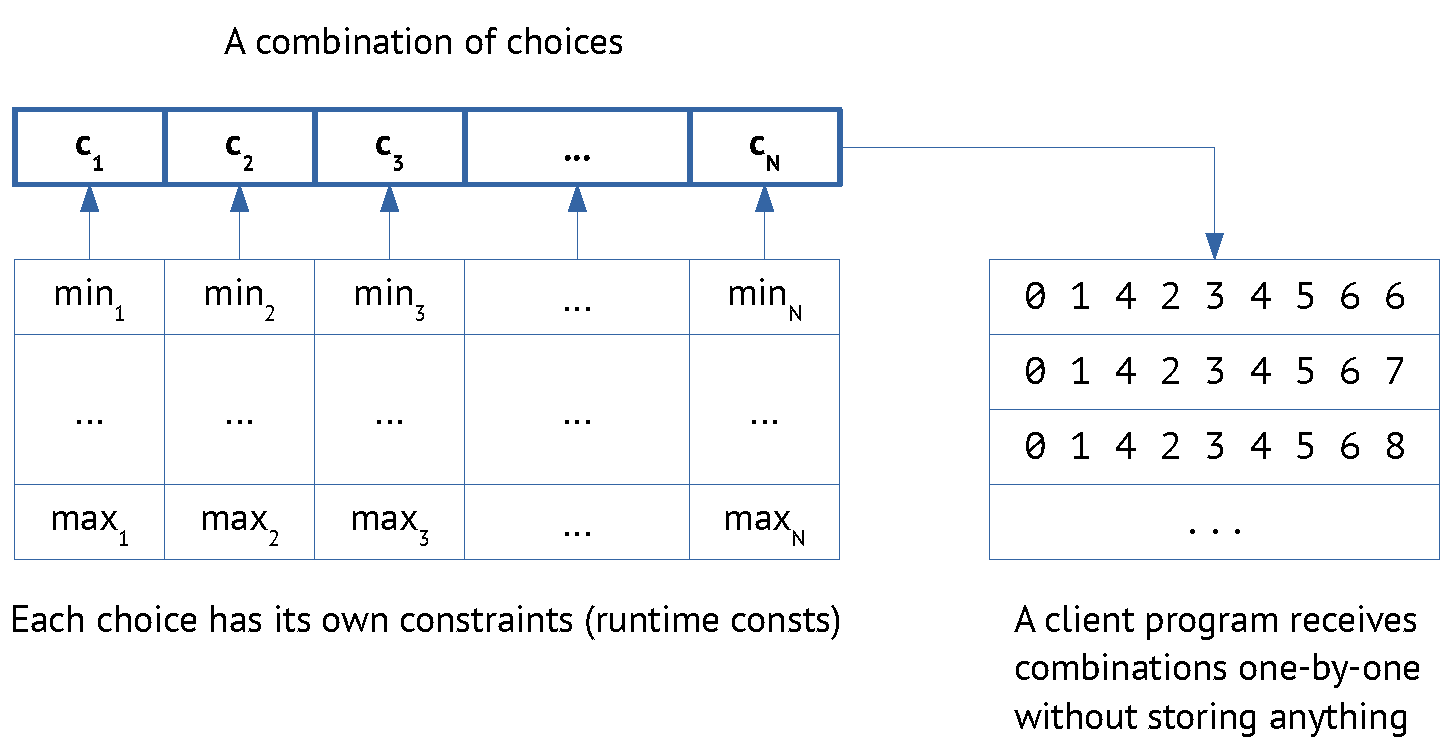
\includegraphics[width=11cm]{figures/combinations}
\end{center}

\end{frame}



\begin{frame}[fragile]{Multi-Iterator: motivation}

TODO Trend link video by Hal Finkel

\end{frame}



\begin{frame}[fragile]{Simple example}

\begin{lstlisting}[basicstyle=\tiny\ttfamily, language=c++]
#include <multiit/multiit.h>

multiit::runtime::MultiIterator mi({ 2, 3, 4 });
// OR: multiit::compiletime::MultiIterator<2, 3, 4> mi;

int niters = 0; 
while (1)       
{               
    niters++;           
                        
    bool next = mi.next();
    if (!next) break;   
                        
    const auto& current = mi.getCurrent();
                        
    // TODO Use the current combination of choices in a target app.
}               

printf("%d iterations visited\n", niters);
\end{lstlisting}

\end{frame}



\begin{frame}[fragile]{Supported types of multi-iterators}

\begin{itemize}
\item \texttt{MultiIterator}: A group of indexes that iterate from 0 to the given upper value
\item \texttt{LimitedMultiIterator}: A group of indexes that iterates only through indexes with total sum no greater than limit
\item \texttt{GenericMultiIterator}: A hosting group of indexes, whose indexes are themselves groups of indexes
\end{itemize}

\vskip20pt

$\Rightarrow$ A \texttt{GenericMultiIterator} of \texttt{MultiIterator} and \texttt{LimitedMultiIterator} elements can be used to express many kinds of combinatorial iterations

\end{frame}



\begin{frame}[fragile]{Programming package structure}

\begin{itemize}
\item \texttt{multiit}: general-purpose multi-iterators in C++, with unit tests
\item \texttt{kernit}: multi-iterator \emph{kernel} generator based on JIT-compilation located in the cloud (web service)
\item \texttt{respyit} : subjected multi-iterators, with Python API, which quiries \texttt{kernit} to provide a kernel with required specifics
\end{itemize}

\end{frame}



\begin{frame}[fragile]{Cloud serivce + end-user application pipeline}

TODO Pipeline figure

\end{frame}



\begin{frame}[fragile]{End-user example}

\begin{lstlisting}[basicstyle=\tiny\ttfamily, language=python]
import respyit

# TODO
\end{lstlisting}

\end{frame}



\end{document}

